%!TEX TS-program = xelatex

\documentclass[t]{beamer}

\usetheme{Hannover}
\usecolortheme{rose}

%%% Работа с русским языком
\usepackage[english,russian]{babel}   %% загружает пакет многоязыковой вёрстки
\usepackage{fontspec,xltxtra,xunicode}      %% подготавливает загрузку шрифтов Open Type, True Type и др.
%\defaultfontfeatures{Ligatures={TeX},Renderer=Basic}  %% свойства шрифтов по умолчанию
\setmainfont[Ligatures={TeX,Historic},
SmallCapsFont={Brill},
SmallCapsFeatures={Letters=SmallCaps}]{Brill} %% задаёт основной шрифт документа
\setsansfont{Brill}                    %% задаёт шрифт без засечек
\setmonofont[Ligatures=NoCommon]{DejaVu Sans}
\newfontfamily\SYM{Brill}
\usepackage{indentfirst}
%%% Дополнительная работа с математикой
\usepackage{amsmath,amsfonts,amssymb,amsthm,mathtools} % AMS
\usepackage{icomma} % "Умная" запятая: $0,2$ --- число, $0, 2$ --- перечисление

%%% Работа с картинками
\usepackage{wrapfig} % Обтекание рисунков текстом
\usepackage{rotating}
\usepackage{fixltx2e}
\usepackage{hhline}
\usepackage{lscape}

%%% Работа с таблицами
\usepackage{array,tabularx,tabulary,booktabs} % Дополнительная работа с таблицами
\usepackage{longtable}  % Длинные таблицы
\usepackage{multirow} % Слияние строк в таблице

\usepackage{multicol} % Несколько колонок

%%% Страница
%\usepackage{fancyhdr} % Колонтитулы
% 	\pagestyle{fancy}
 	%\renewcommand{\headrulewidth}{0pt}  % Толщина линейки, отчеркивающей верхний колонтитул
% 	\lfoot{Нижний левый}
% 	\rfoot{Нижний правый}
% 	\rhead{Верхний правый}
% 	\chead{Верхний в центре}
% 	\lhead{Верхний левый}
%	\cfoot{Нижний в центре} % По умолчанию здесь номер страницы

\usepackage{setspace} % Интерлиньяж
%\onehalfspacing % Интерлиньяж 1.5
%\doublespacing % Интерлиньяж 2
\singlespacing % Интерлиньяж 1

\usepackage{subfig} % подкартинки
\usepackage{lastpage} % Узнать, сколько всего страниц в документе.
\usepackage{soul} % Модификаторы начертания
\usepackage{bbding}
\usepackage{hyperref}
\usepackage{tikz} % Работа с графикой
\usepackage{pgfplots}
\usepackage{pgfplotstable}
\usepackage{verbatim}

\usepackage{attachfile2}
 \attachfilesetup{appearance=true,
color=0 0 0
 }
\usepackage{alltt}

%%% Лингвистические пакеты
%\usepackage{savetrees} % пакет, который экономит место
\usepackage{forest} % для рисования деревьев
\usepackage{vowel} % для рисования трапеций гласных
\usepackage{natbib}
\bibpunct[: ]{[}{]}{;}{a}{}{,}
\usepackage[nogroupskip,nopostdot, nonumberlist]{glossaries}
%\usepackage{glossary-mcols} 
%\setglossarystyle{mcolindex}
\usepackage{philex} % пакет для примеров
\newcommand{\mytem}{\item[$\circ$]}
\addto\captionsrussian{
\renewcommand{\refname}{}}

\newcommand{\apostrophe}{\XeTeXglyph\XeTeXcharglyph"0027\relax}
\usetikzlibrary{patterns}

\usepackage{ulem}
   \newcommand{\code}[1]{\scriptsize \texttt{#1}\normalsize}
   \newcommand{\codel}[1]{\scriptsize \begin{alltt} #1 \end{alltt} \normalsize}   
\setbeamercolor{alerted text}{fg=blue}
\setbeamersize{text margin left=4mm,text margin right=1mm} 
\setbeamertemplate{navigation symbols}{
	\usebeamerfont{footline}%
    \usebeamercolor[fg]{footline}%
    \hspace{1em}%
    {{\small презентация доступна: \href{https://goo.gl/4T12Ar}{\textbf{https://goo.gl/4T12Ar}}}
    \hspace{40mm}
    \insertframenumber/\inserttotalframenumber\vspace{0.5mm}}}
% начало
\title[]{Визуализация данных:\\ базовые функции R и пакет \small\texttt{ggplot2}\normalsize}
\author[]{Г. Мороз}
\date{}
\begin{document}
\frame{\titlepage}
\section{введение}
\begin{frame}{R для визуализации? Совсем не обязательно\dots}
Взято \href{http://czrt.by/notes/dataviz-tools.html}{{\color{red!13!blue}{отсюда}}}. Куча ресурсов, которые скоро устареют.
\begin{multicols}{3}
\scriptsize
\begin{itemize}
{\color{red!13!blue}{\item[\texttt{\symbol{"1F63C}}] \href{http://matplotlib.org/}{\large Matplotlib}}}
{\color{red!13!blue}{\item[\texttt{\symbol{"1F63C}}] \href{http://bokeh.pydata.org/en/latest/}{\large Bokeh}}}
\mytem \href{http://www.anychart.com/}{AnyChart}
\mytem \href{http://www.onlinecharttool.com/}{Chart Tool}
\mytem \href{http://www.chartjs.org/}{Chart.js}
\mytem \href{http://texty.org.ua/mod/datavis/apps/charts/}{Chartbuilder}
\mytem \href{http://quartz.github.io/Chartbuilder/}{Chartbuilder 2.0}
\mytem \href{http://chartgo.com/}{ChartGo}
\mytem \href{https://github.com/chiasm-project/chiasm}{Chiasm}
\mytem \href{http://d3plus.org/}{D3plus}
\mytem \href{https://datahero.com/}{Datahero}
\mytem \href{http://datamatic.io/}{Datamatic}
\mytem \href{http://datavisu.al/}{Datavisual}
\mytem \href{https://datawrapper.de/}{Datawrapper}
\mytem \href{http://www.duarte.com/diagrammer/}{Diagrammer}
\mytem \href{http://www.diychart.com/}{Diychart}
\mytem \href{http://dygraphs.com/}{Dygraphs}
\mytem \href{http://echarts.baidu.com/}{Echarts}
\mytem \href{http://www.humblesoftware.com/envision}{Envision.js}
\mytem \href{https://filtergraph.com/}{filtergraph}
\mytem \href{http://flare.prefuse.org/}{Flare}
\mytem \href{https://developers.google.com/chart/}{Google Charts}
\mytem \href{http://www.highcharts.com/}{Highcharts}
\mytem \href{http://icharts.net/}{iCharts}
\mytem \href{https://infogr.am/}{Infogr.am}
\mytem \href{http://www.jscharts.com/}{JS Charts}
\mytem \href{http://philogb.github.io/jit/}{JavaScript InfoVis Toolkit}
\mytem \href{http://charts.livegap.com/}{Livegap Charts}
\mytem \href{http://idl.cs.washington.edu/projects/lyra/}{Lyra}
\mytem \href{https://plot.ly/}{Plotly}
\item[\texttt{\symbol{"1F63C}}] \href{https://processing.org/}{{\color{red!13!blue}{\large Processing}}}
\mytem \href{http://www.qlik.com/}{Qlik}
\mytem \href{http://raw.densitydesign.org/}{Raw}
\mytem \href{http://go.sap.com/product/analytics/lumira.html}{Lumira}
\mytem \href{https://slemma.com/}{Slemma}
\mytem \href{http://spotfire.tibco.com/five-ways-to-speed-up-data-analysis}{Spotfire}
\mytem \href{https://spritesapp.com/}{Sprites}
\mytem \href{http://www.tableau.com/}{Tableau}
\mytem \href{http://www.dataviz.org/}{VIDI}
\mytem \href{http://vega.github.io/vega/}{Vega}
\mytem \href{http://visage.co/}{Visage}
\mytem \href{https://vizydrop.com/}{Vizydrop}
\mytem \href{http://www.oicweave.org/}{Weave}
\mytem \href{http://www.zingchart.com/}{Zingchart}
\end{itemize}
\end{multicols}
\end{frame}

\begin{frame}{Элементы визуализации}
\begin{itemize}
\mytem система координат
\end{itemize}
\begin{center}
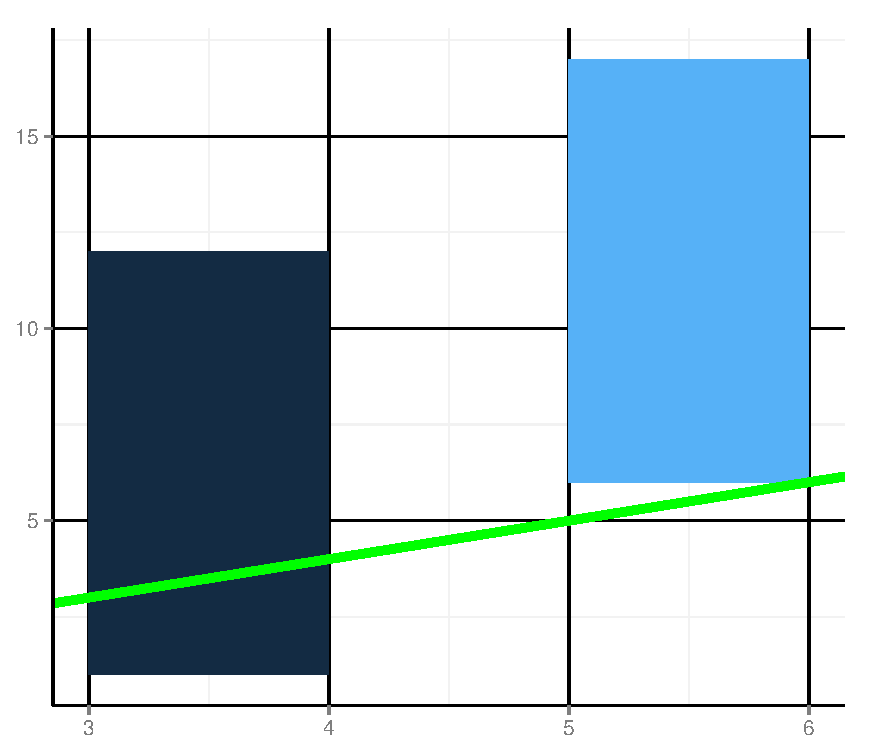
\includegraphics[width=0.3\linewidth]{003-ggplots-coord-1.pdf}\hfill
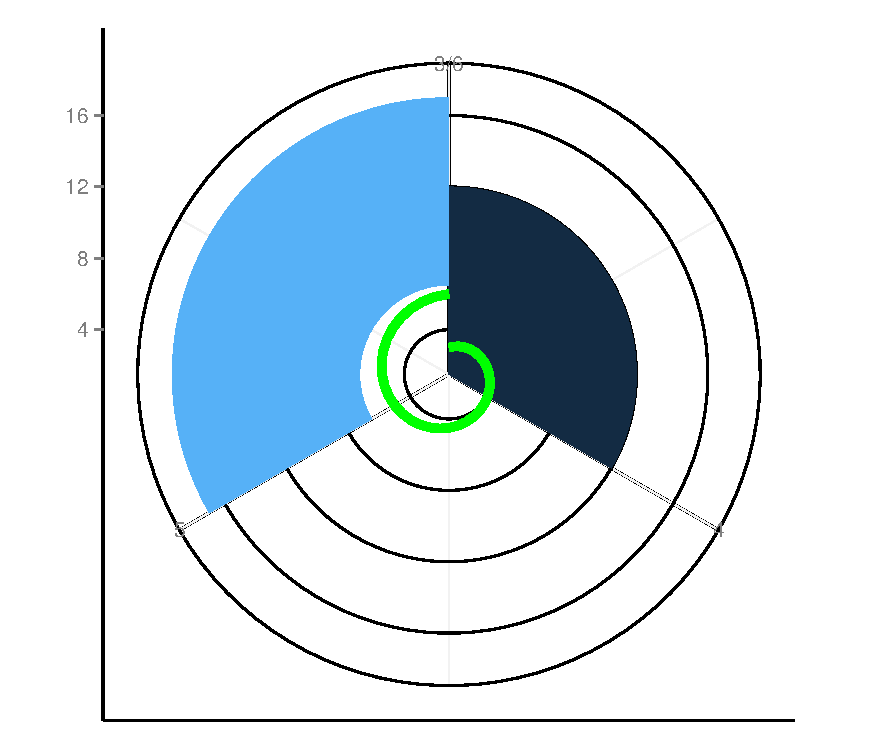
\includegraphics[width=0.3\linewidth]{003-ggplots-coord-2.pdf}\hfill

\includegraphics[width=0.2\linewidth]{003-saggital-slice.pdf}\\ \vspace{-25mm}
\resizebox{0.8\linewidth}{!}{\begin{tikzpicture}[x=1pt,y=1pt]
\definecolor{fillColor}{RGB}{255,255,255}
\path[use as bounding box,fill=fillColor,fill opacity=0.00] (0,0) rectangle (505.89,505.89);
\begin{scope}
\path[clip] ( 25.20,161.59) rectangle (480.69,344.30);
\definecolor{drawColor}{RGB}{0,0,0}
\definecolor{fillColor}{RGB}{190,190,190}

\path[draw=drawColor,line width= 0.4pt,line join=round,line cap=round,fill=fillColor] ( 90.74,306.30) --
	( 93.56,306.53) --
	( 95.71,305.47) --
	( 93.71,305.61) --
	( 96.94,304.17) --
	( 96.26,303.04) --
	( 99.21,304.11) --
	(107.42,301.33) --
	(115.29,296.87) --
	(116.23,294.18) --
	(113.19,290.44) --
	(107.17,289.66) --
	( 95.92,293.21) --
	( 93.23,294.36) --
	( 97.36,290.82) --
	( 96.93,290.51) --
	(100.26,288.46) --
	( 99.34,286.32) --
	(100.44,283.18) --
	(101.83,281.55) --
	(107.19,279.48) --
	(108.23,280.38) --
	(107.44,281.77) --
	(106.35,281.69) --
	(104.80,284.23) --
	(105.99,285.40) --
	(112.53,282.96) --
	(113.85,284.05) --
	(112.41,286.95) --
	(118.90,291.27) --
	(121.57,289.86) --
	(123.01,289.59) --
	(123.71,293.34) --
	(122.16,295.13) --
	(123.16,299.33) --
	(121.38,301.27) --
	(127.26,300.36) --
	(129.20,297.49) --
	(124.95,295.80) --
	(128.25,292.91) --
	(131.68,293.83) --
	(132.08,296.28) --
	(134.52,296.95) --
	(134.43,297.58) --
	(142.66,300.08) --
	(143.68,300.48) --
	(142.95,300.95) --
	(146.78,302.14) --
	(146.39,301.06) --
	(146.56,299.92) --
	(145.79,299.36) --
	(149.07,299.10) --
	(151.94,301.13) --
	(155.35,301.10) --
	(159.40,302.26) --
	(159.67,301.32) --
	(159.37,300.20) --
	(161.42,300.50) --
	(161.31,301.39) --
	(163.83,302.67) --
	(162.23,305.70) --
	(165.86,306.20) --
	(173.54,304.21) --
	(182.23,299.76) --
	(183.78,302.51) --
	(183.26,302.53) --
	(182.61,302.40) --
	(180.09,305.39) --
	(178.42,305.45) --
	(178.40,307.35) --
	(178.93,308.28) --
	(178.93,311.10) --
	(177.85,311.01) --
	(177.83,312.03) --
	(182.48,316.45) --
	(184.39,320.74) --
	(192.71,319.54) --
	(191.41,315.00) --
	(190.41,313.92) --
	(192.44,311.67) --
	(192.10,308.86) --
	(192.38,302.16) --
	(194.60,300.37) --
	(193.58,298.05) --
	(189.93,293.35) --
	(189.19,293.45) --
	(189.61,292.18) --
	(189.13,292.20) --
	(186.95,292.11) --
	(187.28,292.50) --
	(186.56,292.19) --
	(183.66,292.37) --
	(186.70,290.63) --
	(191.51,290.58) --
	(191.75,291.63) --
	(195.31,294.01) --
	(197.49,298.11) --
	(196.55,300.09) --
	(197.00,301.60) --
	(201.93,302.26) --
	(203.52,299.61) --
	(203.68,296.97) --
	(205.71,296.71) --
	(204.15,297.77) --
	(205.22,299.89) --
	(204.02,302.30) --
	(199.05,303.82) --
	(195.05,303.63) --
	(195.19,305.02) --
	(194.57,306.39) --
	(196.35,310.26) --
	(193.37,313.86) --
	(196.78,316.37) --
	(198.24,317.59) --
	(197.70,320.21) --
	(199.49,319.03) --
	(199.59,317.45) --
	(198.63,315.54) --
	(199.04,314.09) --
	(198.83,313.39) --
	(206.51,311.95) --
	(203.16,313.70) --
	(200.71,315.61) --
	(203.04,316.41) --
	(205.88,316.17) --
	(204.03,317.26) --
	(208.78,318.12) --
	(215.24,315.05) --
	(217.88,314.58) --
	(215.66,312.09) --
	(215.67,309.76) --
	(217.16,311.63) --
	(217.55,309.93) --
	(216.91,307.98) --
	(217.70,308.29) --
	(219.26,309.77) --
	(217.84,312.31) --
	(218.77,314.95) --
	(211.78,319.63) --
	(212.02,321.06) --
	(211.15,322.57) --
	(213.75,323.86) --
	(227.27,324.69) --
	(224.33,322.43) --
	(226.51,321.51) --
	(224.76,323.15) --
	(228.42,324.73) --
	(224.77,326.93) --
	(226.94,327.54) --
	(224.48,328.86) --
	(228.22,329.78) --
	(227.21,330.82) --
	(242.77,334.15) --
	(241.44,334.51) --
	(249.04,334.64) --
	(248.46,334.02) --
	(256.83,335.41) --
	(258.05,334.40) --
	(257.85,333.74) --
	(258.38,335.22) --
	(256.05,336.92) --
	(261.06,337.13) --
	(261.25,338.16) --
	(261.95,339.61) --
	(268.98,342.48) --
	(273.53,340.93) --
	(269.02,339.62) --
	(276.86,338.82) --
	(274.39,336.93) --
	(285.82,337.89) --
	(289.78,335.45) --
	(289.97,334.87) --
	(290.57,335.58) --
	(292.52,333.94) --
	(291.55,333.04) --
	(289.75,333.40) --
	(292.17,332.10) --
	(287.66,328.86) --
	(273.85,322.34) --
	(271.94,319.98) --
	(276.72,321.68) --
	(284.06,324.25) --
	(282.51,324.23) --
	(283.75,325.57) --
	(286.10,325.35) --
	(290.06,324.45) --
	(290.25,325.25) --
	(291.29,323.59) --
	(291.08,322.72) --
	(291.59,321.60) --
	(290.86,319.71) --
	(291.13,319.75) --
	(292.34,322.61) --
	(291.65,323.24) --
	(300.88,323.67) --
	(303.67,323.06) --
	(303.61,322.06) --
	(313.97,320.44) --
	(313.78,321.07) --
	(316.11,321.75) --
	(315.73,323.84) --
	(319.08,324.18) --
	(322.27,323.30) --
	(324.05,322.92) --
	(329.03,321.81) --
	(329.43,321.15) --
	(328.51,320.42) --
	(329.59,319.47) --
	(328.21,318.65) --
	(330.30,317.82) --
	(329.15,316.75) --
	(326.94,317.53) --
	(329.59,315.59) --
	(329.87,315.23) --
	(329.12,314.58) --
	(333.36,311.33) --
	(335.53,311.39) --
	(338.34,315.80) --
	(341.71,313.56) --
	(347.31,314.43) --
	(351.21,313.02) --
	(351.95,313.32) --
	(351.17,313.95) --
	(353.63,314.37) --
	(355.90,314.37) --
	(354.49,316.17) --
	(356.37,317.34) --
	(355.11,317.42) --
	(354.04,317.13) --
	(355.08,318.65) --
	(358.41,319.65) --
	(358.01,320.44) --
	(371.20,317.98) --
	(367.66,318.13) --
	(366.49,317.27) --
	(372.59,317.47) --
	(370.65,316.14) --
	(370.97,317.06) --
	(369.93,317.20) --
	(370.04,316.12) --
	(368.18,315.27) --
	(371.53,316.03) --
	(374.12,317.94) --
	(380.35,316.16) --
	(377.85,314.98) --
	(381.63,313.59) --
	(380.95,313.05) --
	(384.63,312.83) --
	(385.22,311.85) --
	(384.64,311.76) --
	(391.09,311.72) --
	(401.51,311.54) --
	(404.57,309.21) --
	(404.26,306.30) --
	(406.93,304.82) --
	(407.93,302.30) --
	(406.75,300.63) --
	(408.47,303.02) --
	(408.40,304.46) --
	(414.26,306.08) --
	(421.86,305.25) --
	(424.23,305.58) --
	(425.54,303.77) --
	(429.14,301.81) --
	(431.40,303.34) --
	(430.39,305.39) --
	(429.47,305.84) --
	(430.16,307.77) --
	(441.85,306.65) --
	(451.52,303.91) --
	(458.11,299.65) --
	(458.49,299.90) --
	(457.54,300.64) --
	(464.86,296.00) --
	(464.53,295.25) --
	(465.76,294.85) --
	(465.77,291.86) --
	(467.38,291.13) --
	(468.12,290.49) --
	(468.07,291.45) --
	(467.54,292.04) --
	(467.50,293.54) --
	(466.79,294.09) --
	(469.52,293.42) --
	(471.32,293.52) --
	(470.29,293.92) --
	(474.29,292.15) --
	(477.87,289.82) --
	(478.01,289.07) --
	(477.21,289.11) --
	(475.42,287.45) --
	(474.43,287.70) --
	(474.76,286.81) --
	(473.25,286.84) --
	(471.39,287.31) --
	(472.08,285.90) --
	(471.57,285.53) --
	(472.00,284.53) --
	(470.79,283.57) --
	(470.92,282.71) --
	(471.76,281.85) --
	(470.94,281.84) --
	(470.43,282.28) --
	(469.64,281.29) --
	(469.35,282.15) --
	(467.87,282.01) --
	(463.43,285.00) --
	(462.79,286.66) --
	(456.87,287.22) --
	(456.07,289.24) --
	(456.65,290.69) --
	(455.47,290.13) --
	(454.89,290.38) --
	(453.80,288.62) --
	(454.86,286.87) --
	(450.13,282.84) --
	(449.69,282.71) --
	(446.54,283.89) --
	(444.61,283.86) --
	(443.71,284.34) --
	(441.37,283.37) --
	(444.30,283.54) --
	(443.91,282.63) --
	(447.13,283.32) --
	(447.05,281.99) --
	(448.83,281.37) --
	(450.21,278.45) --
	(449.56,278.03) --
	(451.66,275.68) --
	(452.02,273.65) --
	(450.77,272.48) --
	(446.87,274.22) --
	(446.05,274.40) --
	(446.38,273.42) --
	(437.22,268.84) --
	(435.88,268.02) --
	(430.22,262.94) --
	(429.35,261.69) --
	(427.10,264.47) --
	(421.60,263.15) --
	(419.62,261.40) --
	(420.11,263.96) --
	(417.00,261.51) --
	(416.29,261.18) --
	(415.00,261.64) --
	(413.64,261.66) --
	(412.61,259.57) --
	(411.09,256.29) --
	(409.43,253.00) --
	(410.67,251.59) --
	(411.28,252.41) --
	(412.42,251.00) --
	(411.38,249.21) --
	(411.77,246.84) --
	(412.55,246.12) --
	(412.42,244.17) --
	(411.57,243.84) --
	(411.26,245.05) --
	(411.66,245.71) --
	(411.16,245.78) --
	(408.86,241.25) --
	(409.79,237.86) --
	(407.41,237.16) --
	(404.48,234.48) --
	(404.54,230.46) --
	(403.66,230.97) --
	(401.36,229.95) --
	(400.95,230.03) --
	(400.61,225.75) --
	(396.70,221.00) --
	(393.86,240.58) --
	(395.11,247.10) --
	(397.29,250.65) --
	(397.06,251.76) --
	(401.48,253.93) --
	(410.18,264.20) --
	(413.31,266.43) --
	(414.33,268.22) --
	(414.11,269.22) --
	(415.09,272.44) --
	(417.79,273.11) --
	(415.01,274.03) --
	(412.55,272.93) --
	(411.98,269.91) --
	(412.30,269.09) --
	(411.77,269.03) --
	(410.48,269.32) --
	(405.37,264.79) --
	(405.59,266.42) --
	(404.38,266.05) --
	(405.44,269.92) --
	(403.44,269.87) --
	(398.52,269.95) --
	(392.44,263.47) --
	(390.59,259.94) --
	(392.88,258.43) --
	(388.31,257.62) --
	(384.50,256.60) --
	(383.08,257.58) --
	(385.85,258.22) --
	(382.75,259.80) --
	(379.49,260.71) --
	(378.24,259.75) --
	(377.30,258.90) --
	(372.59,258.90) --
	(371.30,258.21) --
	(370.22,258.71) --
	(363.81,258.89) --
	(358.45,254.55) --
	(357.25,252.04) --
	(351.62,246.22) --
	(344.46,238.55) --
	(345.96,237.10) --
	(348.06,237.28) --
	(348.07,233.55) --
	(348.80,233.75) --
	(349.17,234.70) --
	(350.03,235.77) --
	(350.00,235.15) --
	(350.78,234.20) --
	(349.55,232.34) --
	(352.38,234.26) --
	(351.79,232.27) --
	(352.28,232.33) --
	(352.92,235.45) --
	(353.87,235.43) --
	(355.33,235.70) --
	(359.45,230.73) --
	(358.20,230.30) --
	(358.69,229.42) --
	(359.07,227.84) --
	(359.47,226.40) --
	(357.72,221.84) --
	(357.35,216.82) --
	(356.86,211.65) --
	(355.46,207.95) --
	(352.00,200.49) --
	(345.08,188.45) --
	(340.75,183.59) --
	(337.34,183.83) --
	(337.41,185.45) --
	(336.35,185.14) --
	(335.12,183.55) --
	(333.57,182.87) --
	(333.51,181.29) --
	(333.00,182.88) --
	(333.69,183.71) --
	(334.68,185.53) --
	(334.18,192.34) --
	(336.10,194.86) --
	(337.18,191.78) --
	(338.64,193.74) --
	(339.78,195.98) --
	(341.79,202.89) --
	(343.15,205.42) --
	(342.83,208.59) --
	(338.15,206.62) --
	(334.17,205.72) --
	(333.11,210.22) --
	(330.94,212.94) --
	(326.42,214.51) --
	(325.69,216.56) --
	(322.02,228.83) --
	(316.52,232.21) --
	(310.84,231.33) --
	(307.95,229.16) --
	(307.84,228.08) --
	(308.30,228.19) --
	(308.69,228.13) --
	(309.04,226.70) --
	(308.67,224.65) --
	(305.68,218.78) --
	(305.83,217.50) --
	(302.25,214.01) --
	(297.52,216.01) --
	(294.18,217.33) --
	(290.63,214.83) --
	(285.13,212.43) --
	(279.74,213.15) --
	(278.09,215.54) --
	(273.09,218.08) --
	(268.96,217.00) --
	(264.81,218.62) --
	(264.01,221.77) --
	(256.27,225.80) --
	(253.72,221.53) --
	(254.55,217.61) --
	(252.82,215.52) --
	(246.19,216.45) --
	(244.99,218.07) --
	(240.54,219.71) --
	(233.60,215.43) --
	(231.99,213.88) --
	(228.45,212.23) --
	(226.38,214.67) --
	(225.78,214.58) --
	(223.55,214.43) --
	(221.38,217.15) --
	(219.22,220.27) --
	(214.15,219.59) --
	(212.45,221.89) --
	(210.39,220.05) --
	(205.80,229.57) --
	(201.63,234.54) --
	(202.37,235.91) --
	(196.69,232.83) --
	(193.96,232.36) --
	(194.81,234.12) --
	(192.19,234.55) --
	(191.53,235.27) --
	(189.12,235.16) --
	(188.67,236.10) --
	(188.28,238.77) --
	(187.05,240.28) --
	(184.64,240.62) --
	(181.56,239.52) --
	(174.29,236.79) --
	(171.44,235.82) --
	(164.80,234.66) --
	(164.23,232.54) --
	(164.99,232.56) --
	(164.55,231.92) --
	(166.46,230.38) --
	(163.73,229.07) --
	(163.94,227.13) --
	(161.72,225.23) --
	(165.34,222.26) --
	(164.94,220.15) --
	(162.01,219.73) --
	(161.10,218.88) --
	(158.31,220.18) --
	(156.01,220.70) --
	(154.29,221.08) --
	(151.66,219.21) --
	(148.53,220.83) --
	(148.52,218.92) --
	(147.07,221.31) --
	(143.14,223.49) --
	(141.56,223.31) --
	(139.72,223.89) --
	(134.17,218.99) --
	(134.29,216.94) --
	(133.84,215.66) --
	(131.67,217.95) --
	(129.94,215.56) --
	(129.84,212.83) --
	(129.00,209.74) --
	(130.90,206.07) --
	(132.23,206.03) --
	(134.72,201.55) --
	(133.74,201.47) --
	(135.27,199.61) --
	(134.06,198.15) --
	(131.23,196.21) --
	(129.26,191.47) --
	(130.01,190.48) --
	(131.08,186.89) --
	(131.32,188.16) --
	(131.20,185.36) --
	(133.55,179.38) --
	(131.88,176.16) --
	(129.02,178.93) --
	(126.77,181.44) --
	(125.60,182.76) --
	(122.91,182.61) --
	(121.08,183.89) --
	(113.14,186.88) --
	(111.76,187.67) --
	(104.80,194.04) --
	(105.18,195.01) --
	(105.90,194.85) --
	(107.22,195.18) --
	(107.13,196.04) --
	(108.83,198.45) --
	(107.61,200.44) --
	(108.63,201.21) --
	(111.10,203.48) --
	(108.60,202.99) --
	(108.58,203.92) --
	(110.26,206.46) --
	(110.89,206.38) --
	(112.11,206.40) --
	(112.66,207.89) --
	(112.37,209.73) --
	(112.70,210.74) --
	(112.34,211.29) --
	(112.67,211.97) --
	(113.08,213.94) --
	(107.36,216.73) --
	(106.06,217.87) --
	(102.42,217.80) --
	(101.53,220.72) --
	( 98.92,221.89) --
	( 98.84,223.30) --
	( 99.27,224.04) --
	( 97.71,226.90) --
	( 93.19,225.66) --
	( 92.13,229.26) --
	( 92.00,230.73) --
	( 92.95,230.56) --
	( 95.21,231.80) --
	( 92.96,233.78) --
	( 90.57,238.01) --
	( 90.72,240.63) --
	( 90.24,241.98) --
	( 87.05,242.56) --
	( 85.70,243.28) --
	( 84.26,244.73) --
	( 82.93,247.38) --
	( 83.19,248.71) --
	( 82.48,250.48) --
	( 83.09,252.22) --
	( 83.55,252.18) --
	( 84.18,252.26) --
	( 82.77,253.45) --
	( 83.15,254.61) --
	( 83.15,256.80) --
	( 83.80,258.58) --
	( 83.88,260.15) --
	( 86.23,261.31) --
	( 88.92,261.18) --
	( 87.10,262.56) --
	( 85.32,264.23) --
	( 83.27,264.20) --
	( 92.36,274.89) --
	( 88.76,278.55) --
	( 89.85,280.06) --
	( 88.89,281.63) --
	( 88.92,282.90) --
	( 88.10,283.63) --
	( 87.95,284.89) --
	( 87.73,285.54) --
	( 87.97,286.67) --
	( 88.86,287.62) --
	( 86.42,292.94) --
	( 88.48,296.12) --
	( 85.13,299.78) --
	( 85.48,302.12) --
	( 89.08,305.20) --
	( 90.54,305.14) --
	( 90.74,306.30) --
	cycle;
\definecolor{fillColor}{RGB}{255,255,255}

\path[draw=drawColor,line width= 0.4pt,line join=round,line cap=round,fill=fillColor] ( 63.35,236.53) --
	( 72.51,235.35) --
	( 73.66,228.36) --
	( 72.09,226.50) --
	( 73.09,224.79) --
	( 73.89,220.75) --
	( 73.97,218.10) --
	( 70.78,213.88) --
	( 70.88,211.86) --
	( 66.94,213.58) --
	( 63.80,213.13) --
	( 62.49,214.01) --
	( 61.48,214.00) --
	( 60.71,215.79) --
	( 60.30,215.91) --
	( 58.75,217.11) --
	( 56.98,218.12) --
	( 56.64,217.08) --
	( 55.44,217.80) --
	( 55.46,218.51) --
	( 52.92,220.08) --
	( 51.91,220.15) --
	( 52.07,221.22) --
	( 51.49,223.17) --
	( 51.41,226.02) --
	( 50.35,228.90) --
	( 50.44,230.01) --
	( 50.38,233.11) --
	( 50.91,232.95) --
	( 50.34,234.13) --
	( 57.66,237.76) --
	( 61.30,237.56) --
	( 60.67,237.82) --
	( 61.08,236.40) --
	( 63.35,236.53) --
	cycle;

\path[draw=drawColor,line width= 0.4pt,line join=round,line cap=round,fill=fillColor] ( 66.86,243.86) --
	( 71.31,245.35) --
	( 76.33,245.03) --
	( 80.28,241.48) --
	( 80.11,240.44) --
	( 80.48,239.92) --
	( 78.23,237.71) --
	( 78.18,235.77) --
	( 78.29,235.62) --
	( 77.71,235.17) --
	( 73.73,234.15) --
	( 71.18,236.24) --
	( 71.20,238.26) --
	( 67.69,240.25) --
	( 66.86,243.86) --
	cycle;

\path[draw=drawColor,line width= 0.4pt,line join=round,line cap=round,fill=fillColor] ( 43.38,257.37) --
	( 41.54,259.15) --
	( 41.39,259.88) --
	( 39.91,257.06) --
	( 39.17,257.07) --
	( 34.84,253.02) --
	( 32.48,252.97) --
	( 32.06,252.96) --
	( 29.12,256.40) --
	( 29.93,257.02) --
	( 30.32,257.15) --
	( 30.40,258.88) --
	( 30.67,259.43) --
	( 28.17,258.23) --
	( 29.14,260.45) --
	( 29.88,260.82) --
	( 31.54,263.61) --
	( 31.56,262.45) --
	( 32.24,264.04) --
	( 29.20,261.34) --
	( 28.10,260.53) --
	( 28.76,262.06) --
	( 29.24,262.48) --
	( 28.26,263.96) --
	( 28.94,264.57) --
	( 28.44,264.35) --
	( 28.08,266.63) --
	( 32.66,266.28) --
	( 33.69,267.32) --
	( 33.52,268.00) --
	( 32.57,267.04) --
	( 31.60,267.42) --
	( 28.11,267.16) --
	( 27.86,268.28) --
	( 28.26,268.78) --
	( 27.81,270.41) --
	( 29.46,270.51) --
	( 28.08,270.98) --
	( 30.48,272.45) --
	( 30.92,272.76) --
	( 32.09,273.77) --
	( 35.37,274.19) --
	( 33.70,274.10) --
	( 32.77,274.18) --
	( 32.07,274.14) --
	( 35.39,275.83) --
	( 35.97,275.61) --
	( 35.80,276.72) --
	( 36.31,277.35) --
	( 37.96,277.99) --
	( 39.85,277.59) --
	( 41.64,277.95) --
	( 42.96,279.41) --
	( 43.18,280.19) --
	( 39.74,278.04) --
	( 39.07,279.03) --
	( 43.16,283.40) --
	( 45.61,284.91) --
	( 46.11,285.41) --
	( 45.16,286.17) --
	( 47.24,289.16) --
	( 46.77,289.53) --
	( 48.15,290.15) --
	( 47.59,290.12) --
	( 48.06,292.27) --
	( 49.01,292.95) --
	( 51.61,294.51) --
	( 52.89,294.79) --
	( 51.14,294.84) --
	( 52.45,296.15) --
	( 53.56,295.65) --
	( 52.90,297.11) --
	( 51.73,297.04) --
	( 52.83,298.00) --
	( 53.13,297.81) --
	( 53.39,297.84) --
	( 53.03,298.19) --
	( 54.23,299.01) --
	( 55.35,297.64) --
	( 55.02,299.46) --
	( 57.84,300.05) --
	( 56.01,300.30) --
	( 57.34,301.33) --
	( 59.64,304.21) --
	( 61.54,304.16) --
	( 60.97,304.71) --
	( 63.55,306.39) --
	( 63.58,305.52) --
	( 65.10,307.03) --
	( 64.42,304.35) --
	( 65.50,305.20) --
	( 66.11,305.10) --
	( 65.83,306.89) --
	( 66.36,306.86) --
	( 69.01,306.44) --
	( 67.72,308.08) --
	( 70.20,308.82) --
	( 72.36,307.57) --
	( 75.02,310.68) --
	( 75.11,311.34) --
	( 76.89,311.25) --
	( 77.38,311.34) --
	( 78.05,311.26) --
	( 76.43,307.94) --
	( 80.51,311.56) --
	( 80.43,309.79) --
	( 82.66,310.94) --
	( 82.14,311.82) --
	( 84.72,311.72) --
	( 83.52,310.37) --
	( 84.29,310.49) --
	( 84.23,309.29) --
	( 85.59,311.11) --
	( 90.96,308.85) --
	( 85.66,307.94) --
	( 87.66,307.18) --
	( 88.12,306.04) --
	( 88.60,306.08) --
	( 90.87,305.70) --
	( 89.55,305.39) --
	( 85.93,303.01) --
	( 87.01,304.88) --
	( 83.88,307.15) --
	( 79.65,306.29) --
	( 78.34,303.08) --
	( 75.99,300.94) --
	( 71.15,301.34) --
	( 68.74,303.43) --
	( 66.87,303.58) --
	( 64.60,302.83) --
	( 65.00,302.43) --
	( 64.24,300.65) --
	( 64.90,300.35) --
	( 60.19,300.71) --
	( 59.76,298.79) --
	( 58.40,298.40) --
	( 55.06,295.92) --
	( 55.65,294.33) --
	( 53.51,291.59) --
	( 53.34,290.47) --
	( 51.05,289.66) --
	( 50.90,285.89) --
	( 48.88,282.61) --
	( 49.42,282.31) --
	( 50.07,280.76) --
	( 47.27,280.20) --
	( 44.87,276.74) --
	( 45.60,272.16) --
	( 45.24,269.59) --
	( 47.01,267.91) --
	( 45.73,266.41) --
	( 46.21,263.37) --
	( 44.58,260.77) --
	( 44.17,257.29) --
	( 43.38,257.37) --
	cycle;

\path[draw=drawColor,line width= 0.4pt,line join=round,line cap=round,fill=fillColor] ( 65.83,302.90) --
	( 66.87,303.58) --
	( 68.74,303.43) --
	( 71.15,301.34) --
	( 75.99,300.94) --
	( 78.34,303.08) --
	( 79.65,306.29) --
	( 83.88,307.15) --
	( 87.01,304.88) --
	( 85.93,303.01) --
	( 84.87,302.15) --
	( 85.59,301.69) --
	( 85.13,299.78) --
	( 88.48,296.12) --
	( 86.42,292.94) --
	( 88.86,287.62) --
	( 87.97,286.67) --
	( 87.73,285.54) --
	( 87.95,284.89) --
	( 88.10,283.63) --
	( 88.92,282.90) --
	( 88.89,281.63) --
	( 89.85,280.06) --
	( 88.76,278.55) --
	( 92.36,274.89) --
	( 83.27,264.20) --
	( 82.46,263.87) --
	( 81.21,263.90) --
	( 80.20,263.64) --
	( 80.11,264.27) --
	( 78.21,262.97) --
	( 78.07,263.27) --
	( 71.66,260.92) --
	( 71.89,261.36) --
	( 71.59,262.20) --
	( 70.30,261.89) --
	( 70.61,262.80) --
	( 67.81,264.47) --
	( 68.01,268.18) --
	( 67.09,273.21) --
	( 68.13,275.93) --
	( 69.95,276.99) --
	( 76.33,283.99) --
	( 76.99,283.85) --
	( 77.32,286.70) --
	( 75.02,288.07) --
	( 73.44,289.94) --
	( 73.76,291.93) --
	( 73.21,294.84) --
	( 72.91,295.67) --
	( 73.15,297.87) --
	( 65.83,302.90) --
	cycle;

\path[draw=drawColor,line width= 0.4pt,line join=round,line cap=round,fill=fillColor] ( 74.82,252.06) --
	( 75.33,254.26) --
	( 74.86,254.39) --
	( 73.47,254.29) --
	( 72.90,255.91) --
	( 72.91,256.21) --
	( 73.17,258.31) --
	( 78.40,260.09) --
	( 83.88,258.70) --
	( 83.52,258.47) --
	( 83.40,258.08) --
	( 81.27,256.68) --
	( 82.97,252.35) --
	( 82.31,251.13) --
	( 80.89,250.78) --
	( 77.86,252.39) --
	( 74.82,252.06) --
	cycle;

\path[draw=drawColor,line width= 0.4pt,line join=round,line cap=round,fill=fillColor] ( 82.19,250.50) --
	( 83.31,248.86) --
	( 82.93,247.38) --
	( 84.26,244.73) --
	( 82.08,242.65) --
	( 81.22,242.69) --
	( 79.41,242.69) --
	( 75.74,245.28) --
	( 72.09,245.22) --
	( 71.90,245.05) --
	( 71.31,245.35) --
	( 66.86,243.86) --
	( 66.82,246.44) --
	( 67.86,249.57) --
	( 70.53,251.40) --
	( 72.31,248.51) --
	( 74.72,248.88) --
	( 74.77,251.67) --
	( 75.93,252.58) --
	( 78.98,251.67) --
	( 82.19,250.50) --
	cycle;

\path[draw=drawColor,line width= 0.4pt,line join=round,line cap=round,fill=fillColor] ( 84.12,244.20) --
	( 87.05,242.56) --
	( 90.24,241.98) --
	( 90.72,240.63) --
	( 90.57,238.01) --
	( 92.96,233.78) --
	( 95.21,231.80) --
	( 92.95,230.56) --
	( 92.00,230.73) --
	( 92.13,229.26) --
	( 92.91,225.80) --
	( 91.90,225.81) --
	( 89.92,223.50) --
	( 89.72,222.03) --
	( 87.54,222.76) --
	( 86.92,222.66) --
	( 85.83,223.24) --
	( 85.34,222.86) --
	( 85.22,223.25) --
	( 83.96,223.35) --
	( 78.72,224.94) --
	( 73.18,223.65) --
	( 73.09,224.79) --
	( 72.09,226.50) --
	( 73.66,228.36) --
	( 72.97,234.08) --
	( 78.18,235.77) --
	( 78.23,237.71) --
	( 80.48,239.92) --
	( 80.01,240.55) --
	( 81.22,242.69) --
	( 82.08,242.65) --
	( 84.12,244.20) --
	cycle;

\path[draw=drawColor,line width= 0.4pt,line join=round,line cap=round,fill=fillColor] ( 92.91,225.80) --
	( 97.91,226.77) --
	( 99.27,224.04) --
	( 98.84,223.30) --
	( 98.92,221.89) --
	(101.53,220.72) --
	(102.42,217.80) --
	(106.06,217.87) --
	(107.36,216.73) --
	(113.08,213.94) --
	(112.67,211.97) --
	(112.34,211.29) --
	(112.70,210.74) --
	(112.37,209.73) --
	(112.66,207.89) --
	(112.11,206.40) --
	(110.89,206.38) --
	(110.26,206.46) --
	(108.58,203.92) --
	(108.51,202.94) --
	(107.66,203.01) --
	(101.75,199.76) --
	(101.49,199.45) --
	(100.40,198.35) --
	(102.14,194.88) --
	(104.46,194.85) --
	(103.35,193.61) --
	(102.90,193.49) --
	(101.93,193.91) --
	( 97.51,190.89) --
	( 97.21,192.01) --
	( 96.87,194.32) --
	( 94.72,195.30) --
	( 97.47,198.17) --
	( 93.11,199.59) --
	( 93.51,199.98) --
	( 92.80,200.55) --
	( 93.80,200.74) --
	( 93.28,202.24) --
	( 92.65,200.94) --
	( 92.27,201.38) --
	( 90.38,199.69) --
	( 88.39,196.89) --
	( 88.19,196.80) --
	( 87.86,196.90) --
	( 87.96,195.03) --
	( 84.54,195.05) --
	( 85.83,197.92) --
	( 86.02,199.95) --
	( 88.23,199.61) --
	( 88.81,199.74) --
	( 87.01,204.28) --
	( 86.71,206.10) --
	( 83.07,209.17) --
	( 79.58,207.64) --
	( 76.08,206.04) --
	( 71.74,207.15) --
	( 69.74,209.00) --
	( 70.49,212.01) --
	( 70.88,211.86) --
	( 70.78,213.88) --
	( 74.26,218.64) --
	( 73.08,223.14) --
	( 75.71,224.83) --
	( 81.99,223.58) --
	( 85.34,222.86) --
	( 85.83,223.24) --
	( 86.92,222.66) --
	( 87.54,222.76) --
	( 89.72,222.03) --
	( 89.92,223.50) --
	( 91.90,225.81) --
	( 92.91,225.80) --
	cycle;

\path[draw=drawColor,line width= 0.4pt,line join=round,line cap=round,fill=fillColor] (128.57,179.31) --
	(128.14,178.00) --
	(129.05,175.98) --
	(128.20,175.96) --
	(125.62,177.18) --
	(121.28,175.96) --
	(119.18,177.80) --
	(116.61,177.61) --
	(117.07,178.47) --
	(117.21,178.98) --
	(116.56,182.81) --
	(112.99,186.57) --
	(118.10,185.30) --
	(122.16,183.01) --
	(124.23,183.15) --
	(124.73,183.21) --
	(126.77,181.44) --
	(128.57,179.31) --
	cycle;

\path[draw=drawColor,line width= 0.4pt,line join=round,line cap=round,fill=fillColor] (128.57,179.31) --
	(131.88,176.16) --
	(134.00,178.84) --
	(136.89,173.33) --
	(138.14,171.98) --
	(136.74,172.01) --
	(135.61,168.92) --
	(135.09,166.54) --
	(134.43,163.59) --
	(133.83,163.47) --
	(132.51,165.85) --
	(133.05,166.60) --
	(132.72,167.57) --
	(133.07,168.19) --
	(131.83,169.10) --
	(131.37,168.62) --
	(131.11,168.42) --
	(128.87,165.71) --
	(128.55,167.09) --
	(128.69,168.31) --
	(126.70,170.50) --
	(127.36,171.18) --
	(126.20,173.13) --
	(126.50,174.37) --
	(125.30,176.15) --
	(125.62,177.18) --
	(128.20,175.96) --
	(129.05,175.98) --
	(128.14,178.00) --
	(128.57,179.31) --
	cycle;

\path[draw=drawColor,line width= 0.4pt,line join=round,line cap=round,fill=fillColor] (299.36,215.43) --
	(296.62,206.87) --
	(297.88,206.17) --
	(301.48,206.24) --
	(303.94,206.87) --
	(307.14,201.62) --
	(305.39,200.93) --
	(302.74,201.05) --
	(301.00,199.80) --
	(298.57,198.46) --
	(296.92,195.55) --
	(294.02,194.70) --
	(291.14,192.52) --
	(287.73,193.76) --
	(286.73,190.15) --
	(287.68,187.46) --
	(284.16,183.51) --
	(279.58,181.76) --
	(278.67,181.84) --
	(272.21,179.15) --
	(269.74,178.25) --
	(269.27,179.11) --
	(267.82,178.68) --
	(262.97,181.93) --
	(249.91,183.67) --
	(247.48,189.80) --
	(241.27,193.63) --
	(239.77,193.63) --
	(236.35,195.15) --
	(236.65,197.66) --
	(236.61,202.36) --
	(234.27,206.42) --
	(231.03,208.13) --
	(231.01,208.57) --
	(229.49,210.61) --
	(229.18,212.04) --
	(230.95,213.87) --
	(233.60,215.43) --
	(240.00,219.76) --
	(244.40,218.84) --
	(245.19,217.05) --
	(251.84,215.14) --
	(254.55,217.61) --
	(253.54,221.02) --
	(256.00,225.65) --
	(263.61,222.52) --
	(264.43,219.50) --
	(266.84,217.14) --
	(271.41,218.19) --
	(277.73,216.05) --
	(278.33,214.38) --
	(283.10,212.61) --
	(289.18,214.10) --
	(293.01,217.16) --
	(295.51,216.50) --
	(299.36,215.43) --
	cycle;

\path[draw=drawColor,line width= 0.4pt,line join=round,line cap=round,fill=fillColor] (135.38,199.55) --
	(133.74,201.47) --
	(134.72,201.55) --
	(132.23,206.03) --
	(130.90,206.07) --
	(129.00,209.74) --
	(129.84,212.83) --
	(129.94,215.56) --
	(131.67,217.95) --
	(133.84,215.66) --
	(134.29,216.94) --
	(134.17,218.99) --
	(139.72,223.89) --
	(141.56,223.31) --
	(143.14,223.49) --
	(147.07,221.31) --
	(148.52,218.92) --
	(148.53,220.83) --
	(151.66,219.21) --
	(154.29,221.08) --
	(156.01,220.70) --
	(158.31,220.18) --
	(161.10,218.88) --
	(162.01,219.73) --
	(164.94,220.15) --
	(165.34,222.26) --
	(161.72,225.23) --
	(163.94,227.13) --
	(163.73,229.07) --
	(166.46,230.38) --
	(164.55,231.92) --
	(164.99,232.56) --
	(164.23,232.54) --
	(164.80,234.66) --
	(171.44,235.82) --
	(174.29,236.79) --
	(181.56,239.52) --
	(184.64,240.62) --
	(187.05,240.28) --
	(188.28,238.77) --
	(188.67,236.10) --
	(189.12,235.16) --
	(191.53,235.27) --
	(192.19,234.55) --
	(194.81,234.12) --
	(193.96,232.36) --
	(196.69,232.83) --
	(202.37,235.91) --
	(201.63,234.54) --
	(205.80,229.57) --
	(210.39,220.05) --
	(212.45,221.89) --
	(214.15,219.59) --
	(219.22,220.27) --
	(221.38,217.15) --
	(223.55,214.43) --
	(225.78,214.58) --
	(226.38,214.67) --
	(227.76,212.16) --
	(227.32,212.18) --
	(226.61,211.04) --
	(225.41,209.19) --
	(223.86,208.05) --
	(223.51,202.86) --
	(221.53,202.45) --
	(220.20,202.47) --
	(217.52,203.22) --
	(215.89,196.52) --
	(216.49,194.45) --
	(214.53,194.50) --
	(210.06,193.21) --
	(211.06,192.42) --
	(211.04,191.43) --
	(211.95,185.61) --
	(211.28,184.07) --
	(210.79,183.44) --
	(210.80,181.06) --
	(206.88,183.58) --
	(199.68,183.59) --
	(196.48,185.18) --
	(194.91,184.76) --
	(194.36,181.67) --
	(190.29,183.55) --
	(188.31,181.90) --
	(185.05,178.32) --
	(182.36,174.19) --
	(181.72,173.69) --
	(181.28,175.39) --
	(178.13,175.90) --
	(177.40,179.30) --
	(176.17,179.83) --
	(176.36,183.78) --
	(175.91,183.97) --
	(173.92,186.97) --
	(166.15,186.99) --
	(162.02,192.48) --
	(161.75,194.88) --
	(161.00,196.10) --
	(161.17,197.43) --
	(162.33,197.40) --
	(164.64,199.61) --
	(163.11,201.30) --
	(161.58,200.57) --
	(163.56,199.13) --
	(161.63,198.58) --
	(160.53,199.54) --
	(160.78,198.64) --
	(160.22,196.70) --
	(159.92,197.72) --
	(158.29,196.72) --
	(152.08,193.57) --
	(151.78,176.72) --
	(151.05,176.52) --
	(149.65,178.16) --
	(146.99,181.34) --
	(143.31,178.81) --
	(143.56,183.27) --
	(140.52,185.12) --
	(139.53,188.72) --
	(138.40,190.26) --
	(137.97,191.56) --
	(139.80,191.33) --
	(140.59,191.38) --
	(139.82,192.61) --
	(140.69,195.10) --
	(144.73,194.87) --
	(144.15,195.73) --
	(144.27,197.02) --
	(144.88,201.40) --
	(143.05,202.22) --
	(140.39,203.01) --
	(135.38,199.55) --
	cycle;

\node[text=drawColor,anchor=base,inner sep=0pt, outer sep=0pt, scale=  1.70] at (258.05,263.56) {Россия};
\end{scope}
\begin{scope}
\path[clip] (  0.00,  0.00) rectangle (505.89,505.89);
\definecolor{drawColor}{RGB}{0,0,0}

\path[draw=drawColor,line width= 0.4pt,line join=round,line cap=round] (137.25,161.59) -- (380.36,161.59);

\path[draw=drawColor,line width= 0.4pt,line join=round,line cap=round] (137.25,161.59) -- (137.25,155.59);

\path[draw=drawColor,line width= 0.4pt,line join=round,line cap=round] (258.80,161.59) -- (258.80,155.59);

\path[draw=drawColor,line width= 0.4pt,line join=round,line cap=round] (380.36,161.59) -- (380.36,155.59);

\node[text=drawColor,anchor=base,inner sep=0pt, outer sep=0pt, scale=  0.80] at (137.25,139.99) {50};

\node[text=drawColor,anchor=base,inner sep=0pt, outer sep=0pt, scale=  0.80] at (258.80,139.99) {100};

\node[text=drawColor,anchor=base,inner sep=0pt, outer sep=0pt, scale=  0.80] at (380.36,139.99) {150};

\path[draw=drawColor,line width= 0.4pt,line join=round,line cap=round] ( 25.20,170.70) -- ( 25.20,307.28);

\path[draw=drawColor,line width= 0.4pt,line join=round,line cap=round] ( 25.20,170.70) -- ( 19.20,170.70);

\path[draw=drawColor,line width= 0.4pt,line join=round,line cap=round] ( 25.20,216.23) -- ( 19.20,216.23);

\path[draw=drawColor,line width= 0.4pt,line join=round,line cap=round] ( 25.20,261.76) -- ( 19.20,261.76);

\path[draw=drawColor,line width= 0.4pt,line join=round,line cap=round] ( 25.20,307.28) -- ( 19.20,307.28);

\node[text=drawColor,anchor=base east,inner sep=0pt, outer sep=0pt, scale=  0.80] at ( 13.20,167.95) {40};

\node[text=drawColor,anchor=base east,inner sep=0pt, outer sep=0pt, scale=  0.80] at ( 13.20,213.47) {50};

\node[text=drawColor,anchor=base east,inner sep=0pt, outer sep=0pt, scale=  0.80] at ( 13.20,259.00) {60};

\node[text=drawColor,anchor=base east,inner sep=0pt, outer sep=0pt, scale=  0.80] at ( 13.20,304.53) {70};

\path[draw=drawColor,line width= 0.4pt,line join=round,line cap=round] ( 25.20,161.59) --
	(480.69,161.59) --
	(480.69,344.30) --
	( 25.20,344.30) --
	( 25.20,161.59);
\end{scope}
\begin{scope}
\path[clip] ( 25.20,161.59) rectangle (480.69,344.30);
\definecolor{drawColor}{gray}{0.80}

\path[draw=drawColor,line width= 0.4pt,line join=round,line cap=round] ( 25.20,170.70) -- (480.69,170.70);

\path[draw=drawColor,line width= 0.4pt,line join=round,line cap=round] ( 25.20,216.23) -- (480.69,216.23);

\path[draw=drawColor,line width= 0.4pt,line join=round,line cap=round] ( 25.20,261.76) -- (480.69,261.76);

\path[draw=drawColor,line width= 0.4pt,line join=round,line cap=round] ( 25.20,307.28) -- (480.69,307.28);

\path[draw=drawColor,line width= 0.4pt,line join=round,line cap=round] ( 25.20,352.81) -- (480.69,352.81);

\path[draw=drawColor,line width= 0.4pt,line join=round,line cap=round] ( 15.69,161.59) -- ( 15.69,344.30);

\path[draw=drawColor,line width= 0.4pt,line join=round,line cap=round] ( 64.32,161.59) -- ( 64.32,344.30);

\path[draw=drawColor,line width= 0.4pt,line join=round,line cap=round] (112.94,161.59) -- (112.94,344.30);

\path[draw=drawColor,line width= 0.4pt,line join=round,line cap=round] (161.56,161.59) -- (161.56,344.30);

\path[draw=drawColor,line width= 0.4pt,line join=round,line cap=round] (210.18,161.59) -- (210.18,344.30);

\path[draw=drawColor,line width= 0.4pt,line join=round,line cap=round] (258.80,161.59) -- (258.80,344.30);

\path[draw=drawColor,line width= 0.4pt,line join=round,line cap=round] (307.42,161.59) -- (307.42,344.30);

\path[draw=drawColor,line width= 0.4pt,line join=round,line cap=round] (356.05,161.59) -- (356.05,344.30);

\path[draw=drawColor,line width= 0.4pt,line join=round,line cap=round] (404.67,161.59) -- (404.67,344.30);

\path[draw=drawColor,line width= 0.4pt,line join=round,line cap=round] (453.29,161.59) -- (453.29,344.30);

\path[draw=drawColor,line width= 0.4pt,line join=round,line cap=round] (501.91,161.59) -- (501.91,344.30);
\definecolor{drawColor}{RGB}{0,0,0}
\definecolor{fillColor}{RGB}{0,0,0}

\path[draw=drawColor,line width= 0.4pt,line join=round,line cap=round,fill=fillColor] (107.15,242.43) circle (  1.50);

\node[text=drawColor,anchor=base west,inner sep=0pt, outer sep=0pt, scale=  1.00] at (113.15,240.14) {Москва};

\path[draw=drawColor,line width= 0.4pt,line join=round,line cap=round,fill=fillColor] (131.13,184.21) circle (  1.50);

\node[text=drawColor,anchor=base,inner sep=0pt, outer sep=0pt, scale=  1.00] at (131.13,172.47) {Махачкала};

\path[draw=drawColor,line width= 0.4pt,line join=round,line cap=round,fill=fillColor] (113.20,191.69) circle (  1.50);

\node[text=drawColor,anchor=base east,inner sep=0pt, outer sep=0pt, scale=  1.00] at (107.20,189.40) {Майкоп};

\path[draw=drawColor,line width= 0.4pt,line join=round,line cap=round] (368.20,184.36) --
	(368.20,178.36) --
	(368.20,184.36) --
	(398.09,184.36) --
	(398.09,178.36) --
	(398.09,184.36) --
	(427.98,184.36) --
	(427.98,178.36) --
	(427.98,184.36) --
	(457.86,184.36) --
	(457.86,178.36);

\node[text=drawColor,anchor=base,inner sep=0pt, outer sep=0pt, scale=  0.60] at (368.50,170.29) {0};

\node[text=drawColor,anchor=base,inner sep=0pt, outer sep=0pt, scale=  0.60] at (399.29,170.29) {1000};

\node[text=drawColor,anchor=base,inner sep=0pt, outer sep=0pt, scale=  0.60] at (429.18,170.29) {2000};

\node[text=drawColor,anchor=base,inner sep=0pt, outer sep=0pt, scale=  0.60] at (460.08,170.29) {3000 km};

\node[text=drawColor,anchor=base west,inner sep=0pt, outer sep=0pt, scale=  0.60] at (368.20,188.88) {scale approx 1:95,000,000};
\end{scope}
\end{tikzpicture}}
\end{center}
\end{frame}

\begin{frame}{Элементы визуализации}
\begin{itemize}
\mytem позиция
\mytem длина
\mytem форма
\mytem угол
\mytem направление
\mytem размер
\mytem цвет
\mytem \dots
\end{itemize}
\end{frame}
\begin{frame}{Данные}
В данной презентации все примеры будут приводиться на примере датасета из работы [Chi-kuk 2007] (доступна по ссылке http://goo.gl/Zjr9aF). В работе исследовались речь 7 гомосексуальных и 7 гетеросексуальных носителей кантонского диалекта языка юэ. В датасете есть следующие переменные:
\begin{itemize}
\mytem долгота s (s.duration.ms)
\mytem долгота гласных (vowel.duration.ms)
\mytem среднее значении ЧОТ (average.f0.Hz)
\mytem диапозон ЧОТ (f0.range.Hz)
\mytem сколько носителей воспринимает говорящего как гомосексуалa (perceived.as.homo)
\mytem сколько носителей воспринимает говорящего как гетеросексуалa (perceived.as.hetero)
\mytem ориентация говорящего (orientation)
\mytem возраст говорящего (age)
\end{itemize}
\end{frame}
\begin{frame}
В R визуализация реализована по-разному:
\begin{itemize}
\item core R (всегда будет слева)
\item библиотекой \code{ggplot2} (всегда будет справа)
\end{itemize}
Все примеры \code{ggplot2} в данной презентации реализованы в связке с пакетом \code{dplyr}. Так что, для того чтобы код из данной презентации работал следует включить библиотеки и скачать датасет:
\codel{
library(ggplot2)\\
library(dplyr)\\
chi.kuk <- read.csv("http://goo.gl/Zjr9aF") \hfill \# закачивает датасет}
\end{frame}
\section{2 переменные}
\subsection{колич+колич}
\begin{frame}{scaterplot}
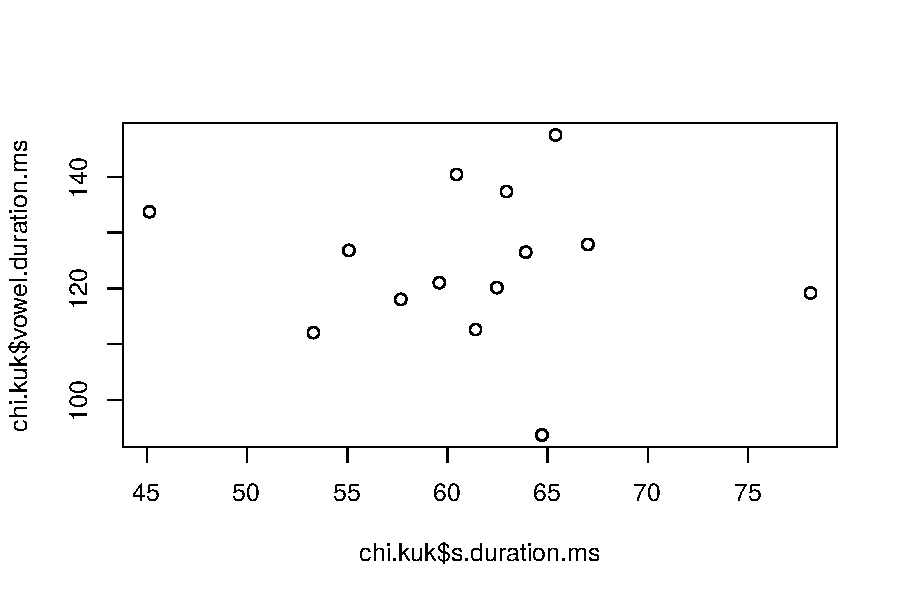
\includegraphics[width=0.49\linewidth]{007-base-scaterplot.pdf}~
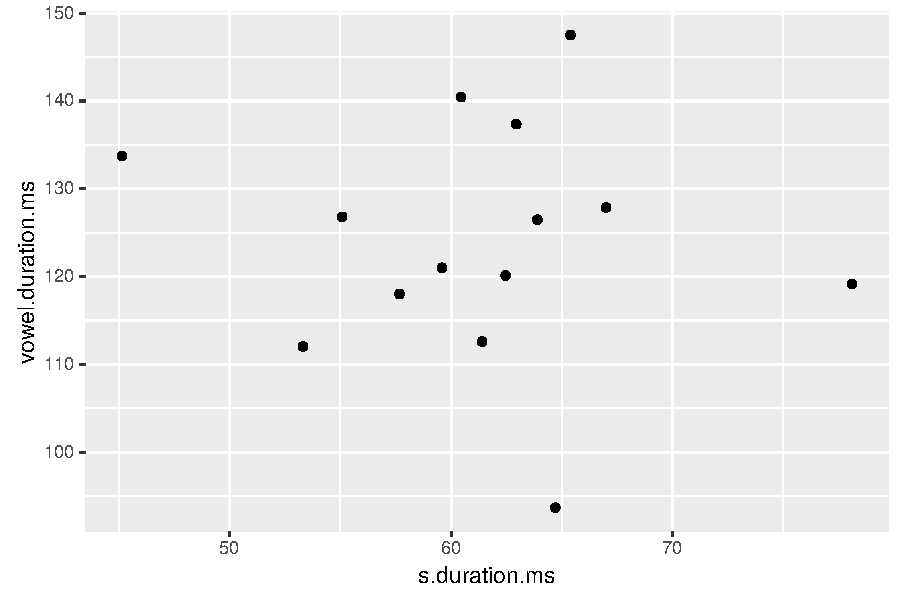
\includegraphics[width=0.49\linewidth]{007-ggplot-scaterplot.pdf}
\codel{
\# base R\\
plot(chi.kuk\$s.duration.ms, chi.kuk\$vowel.duration.ms)\bigskip\\
\# dplyr, ggplot2\\
chi.kuk \%>\% \\
\ \ \ ggplot(aes(s.duration.ms, vowel.duration.ms)) +\\
\ \ \ geom\_point()\\
}
\end{frame}
\begin{frame}{scaterplot: цвет}
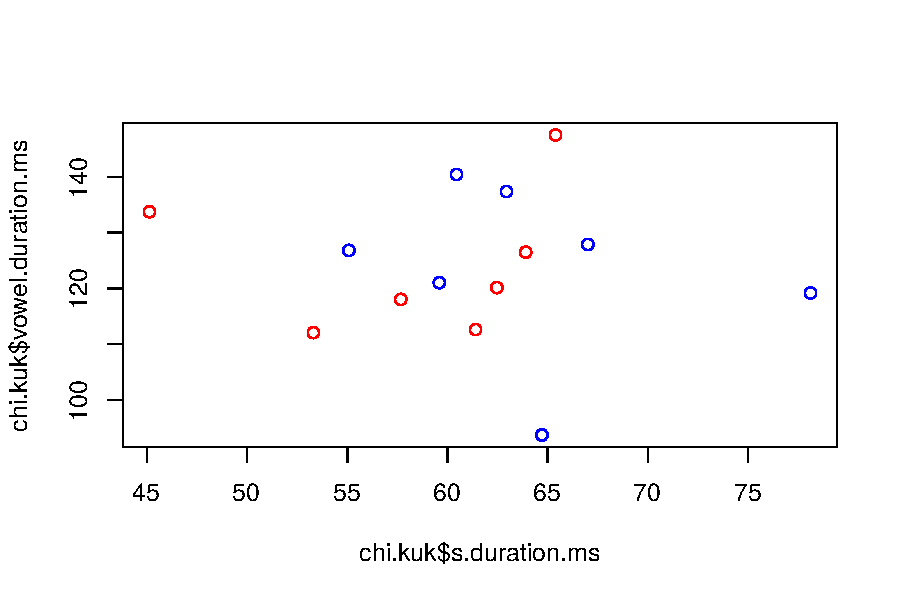
\includegraphics[width=0.49\linewidth]{008-base-scaterplot-color.pdf}~
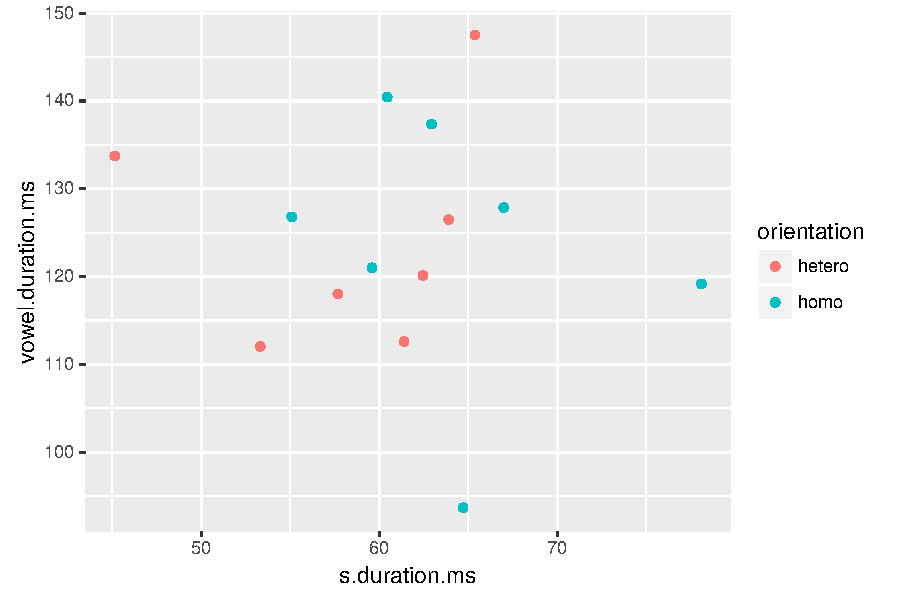
\includegraphics[width=0.49\linewidth]{008-ggplot-scaterplot-color.pdf}
\codel{
\# base R\\
plot(chi.kuk\$s.duration.ms, chi.kuk\$vowel.duration.ms,\\
\ \ \ \alert{col = c("red"{}, "blue")[as.numeric(chi.kuk\$orientation)])})\bigskip\\
\# dplyr, ggplot2\\
chi.kuk \%>\% \\
\ \ \ ggplot(aes(s.duration.ms, vowel.duration.ms, \alert{color = orientation})) +\\
\ \ \ geom\_point()\\
}
\end{frame}
\begin{frame}{scaterplot: форма}
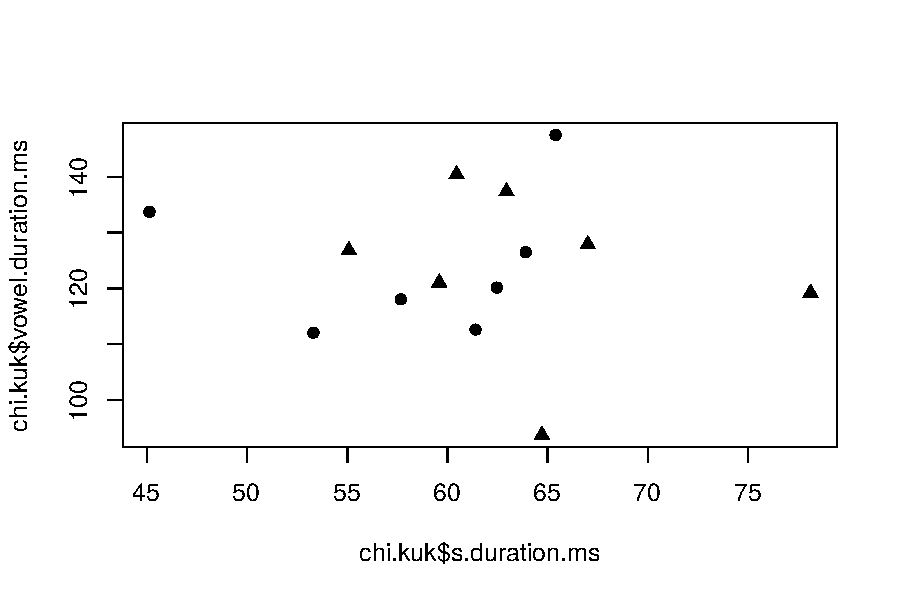
\includegraphics[width=0.49\linewidth]{009-base-scaterplot-shape.pdf}~
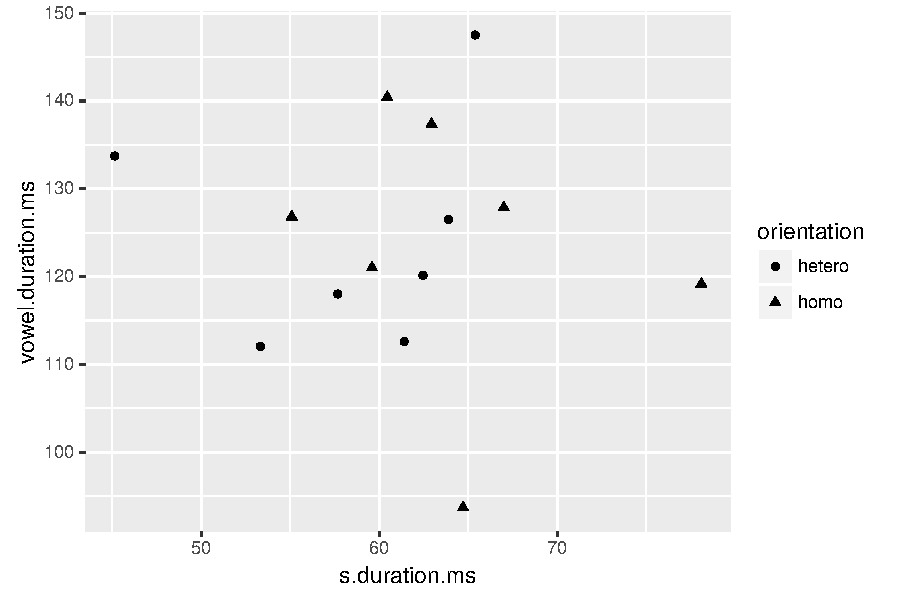
\includegraphics[width=0.49\linewidth]{009-ggplot-scaterplot-shape.pdf}
\codel{
\# base R\\
plot(chi.kuk\$s.duration.ms, chi.kuk\$vowel.duration.ms,\\
\ \ \ \alert{pch = c(16, 17)[as.numeric(chi.kuk\$orientation)])})\bigskip\\
\# dplyr, ggplot2\\
chi.kuk \%>\% \\
\ \ \ ggplot(aes(s.duration.ms, vowel.duration.ms, \alert{shape = orientation})) +\\
\ \ \ geom\_point()\\
}
\end{frame}
\begin{frame}{scaterplot: размер}
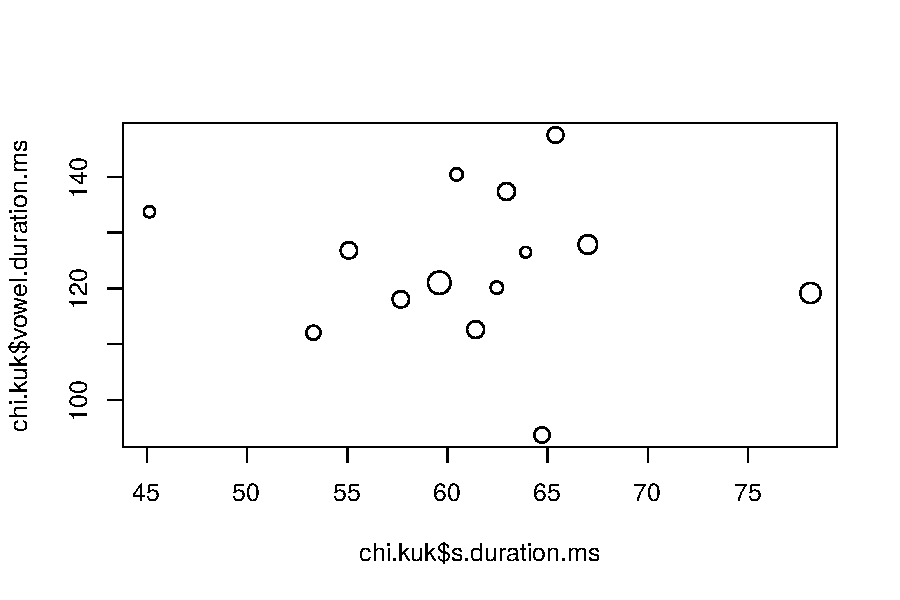
\includegraphics[width=0.49\linewidth]{010-base-scaterplot-size.pdf}~
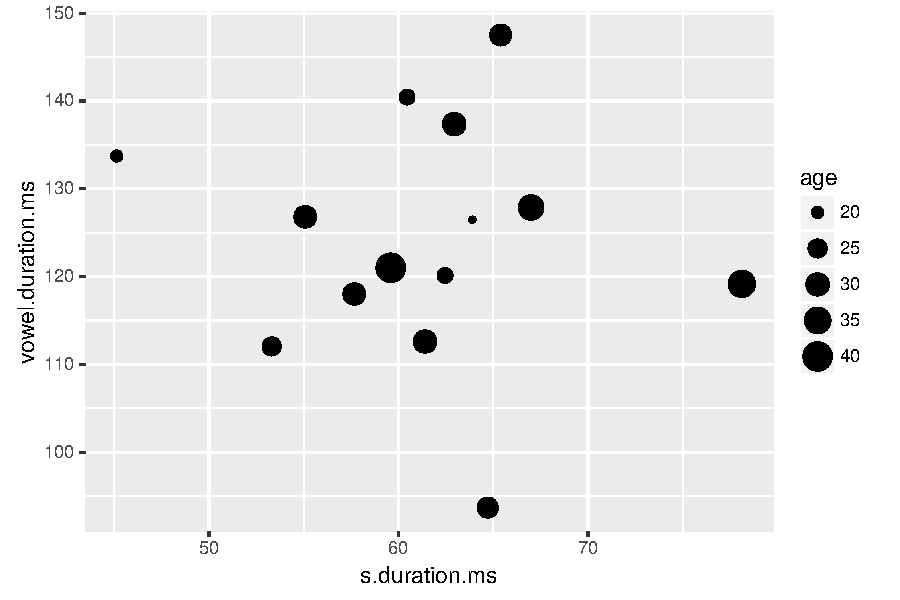
\includegraphics[width=0.49\linewidth]{010-ggplot-scaterplot-size.pdf}
\codel{
\# base R\\
plot(chi.kuk\$s.duration.ms, chi.kuk\$vowel.duration.ms,\\
\ \ \ \alert{cex = chi.kuk\$age/20})\bigskip\\
\# dplyr, ggplot2\\
chi.kuk \%>\% \\
\ \ \ ggplot(aes(s.duration.ms, vowel.duration.ms, \alert{color = orientation})) +\\
\ \ \ geom\_point()\\
}
\end{frame}
\begin{frame}{scaterplot: текст}
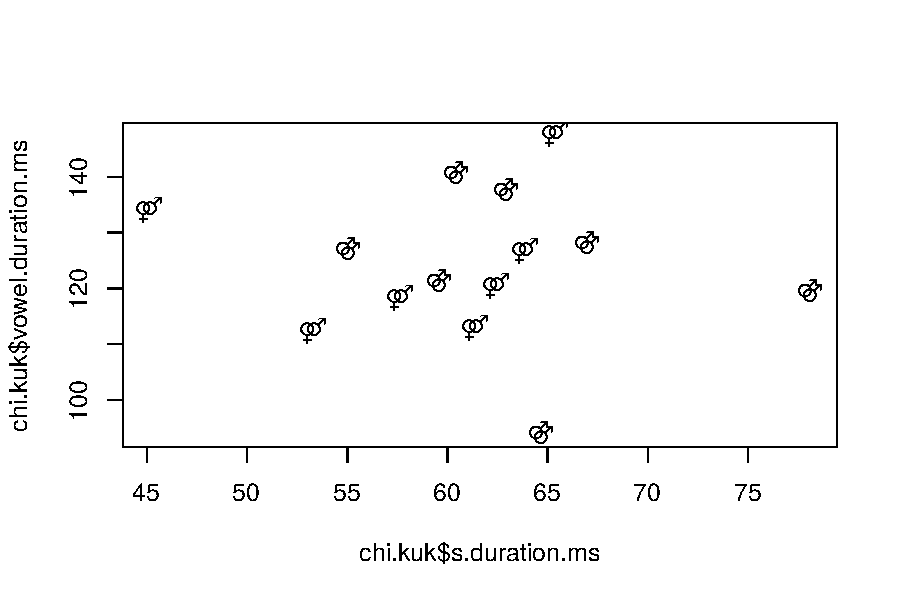
\includegraphics[width=0.49\linewidth]{011-base-scaterplot-text.pdf}~
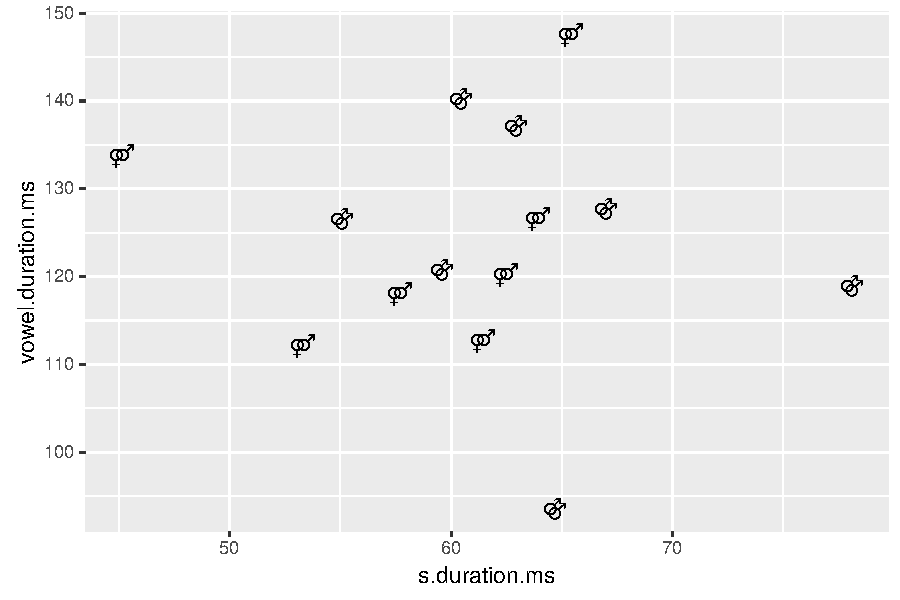
\includegraphics[width=0.49\linewidth]{011-ggplot-scaterplot-text.pdf}
\codel{
\# base R\\
plot(chi.kuk\$s.duration.ms, chi.kuk\$vowel.duration.ms,\\
\ \ \ \alert{pch = c("⚤"{}, "⚣")[as.numeric(chi.kuk\$orientation)])})\bigskip\\
\# dplyr, ggplot2\\
\alert{levels(chi.kuk\$orientation) <- list("homo"{}="⚣"{}, "hetero"{}="⚤")\\}
chi.kuk \%>\% \\
\ \ \ ggplot(aes(s.duration.ms, vowel.duration.ms, \alert{label = orientation})) +\\
\ \ \ \alert{geom\_text()}\\
}
\end{frame}
\begin{frame}{scaterplot: заголовок}
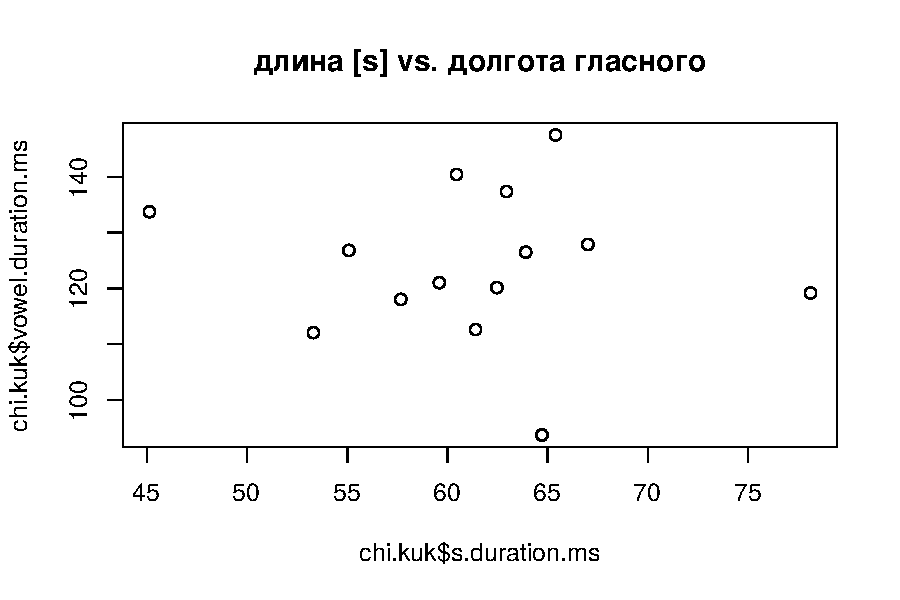
\includegraphics[width=0.49\linewidth]{012-base-scaterplot-title.pdf}~
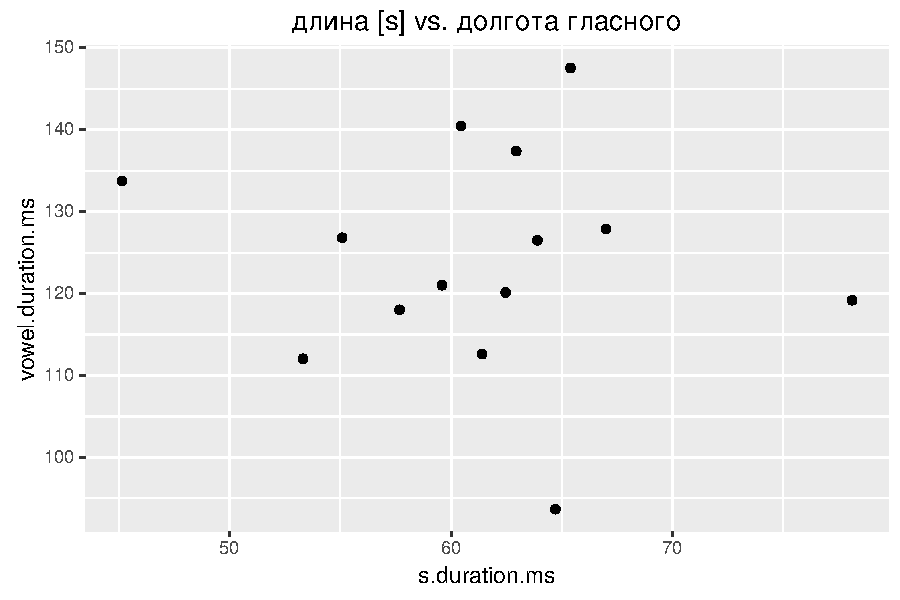
\includegraphics[width=0.49\linewidth]{012-ggplot-scaterplot-title.pdf}
\codel{
\# base R\\
plot(chi.kuk\$s.duration.ms, chi.kuk\$vowel.duration.ms,\\
\ \ \ \alert{main = "длина [s] vs. долгота гласного"})\bigskip\\
\# dplyr, ggplot2\\
chi.kuk \%>\% \\
\ \ \ ggplot(aes(s.duration.ms, vowel.duration.ms)) +\\
\ \ \ geom\_point() +\\
\ \ \ \alert{ggtitle("длина [s] vs. долгота гласного")} \\
}
\end{frame}
\begin{frame}{scaterplot: подписи осей}
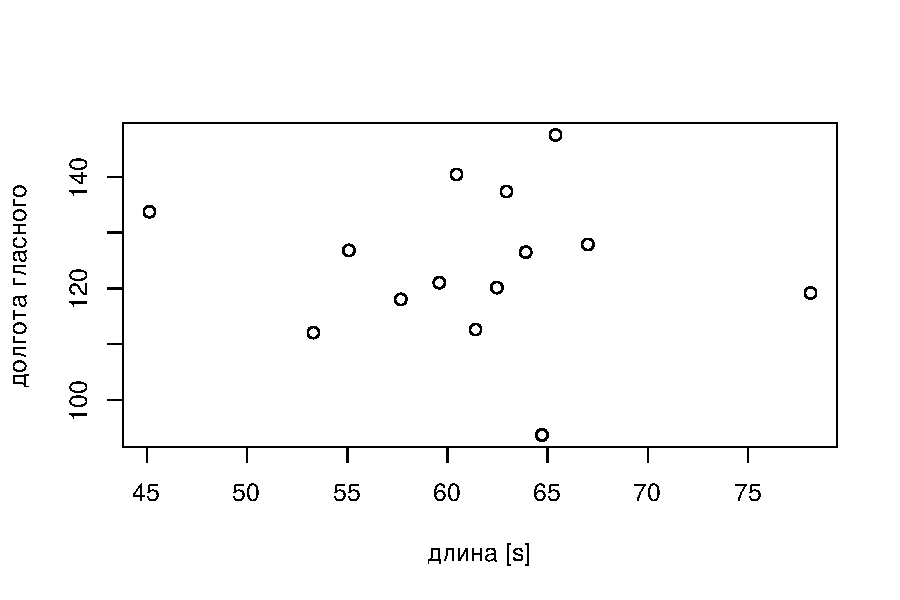
\includegraphics[width=0.49\linewidth]{013-base-scaterplot-axes.pdf}~
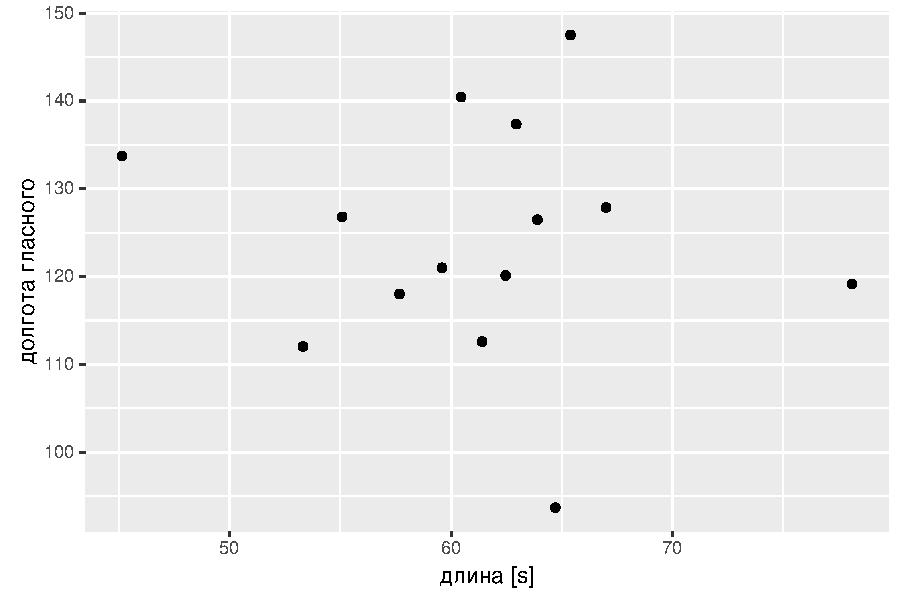
\includegraphics[width=0.49\linewidth]{013-ggplot-scaterplot-axes.pdf}
\codel{
\# base R\\
plot(chi.kuk\$s.duration.ms, chi.kuk\$vowel.duration.ms,\\
\ \ \ \alert{xlab = "длина [s]", ylab = "долгота гласного"})\bigskip\\
\# dplyr, ggplot2\\
chi.kuk \%>\% \\
\ \ \ ggplot(aes(s.duration.ms, vowel.duration.ms)) +\\
\ \ \ geom\_point() +\\
\ \ \ \alert{xlab("длина [s]")+\\
\ \ \ ylab("долгота гласного")} 
}
\end{frame}
\begin{frame}
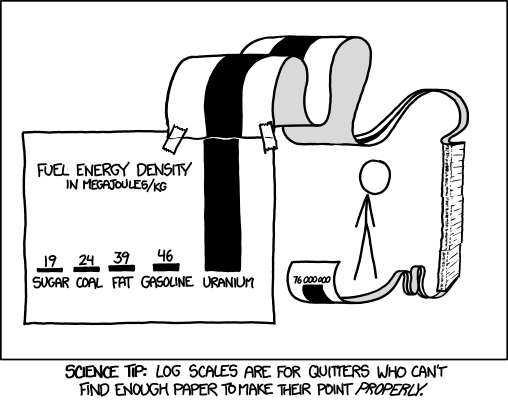
\includegraphics[width=\linewidth]{014-log-scales.png}
\end{frame}
\begin{frame}{scaterplot: логарифмирование осей}
Воспользуемся частотным словарем [Ляшевская, Шаров 2009] (топ-50000 лемм СЛРЯ) и посмотрим на параметр частоты слова (Freq.imp., среднее на миллион словоупотреблений).
\
\codel{
freq <- read.csv("https://goo.gl/TlX7xW"{}, sep = "\textbackslash t")\\}
Если оси не логарифмировать, то получится следующее:
\begin{multicols}{2}
\codel{
freq \%>\% \\
\ \ \ ggplot(aes(1:52138, Freq.ipm.)) +\\
\ \ \ geom\_point() +\\
\ \ \ xlab("{}") +\\
\ \ \ ylab("ipm") 
\columnbreak\\
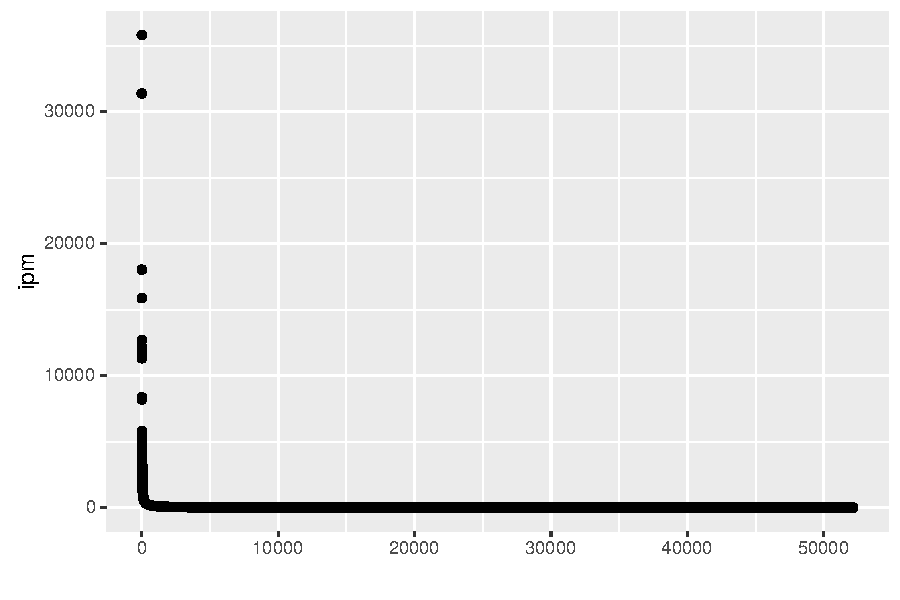
\includegraphics[width=\linewidth]{015-log-scales.pdf}
}
\end{multicols}
\end{frame}
\begin{frame}{scaterplot: логарифмирование осей}
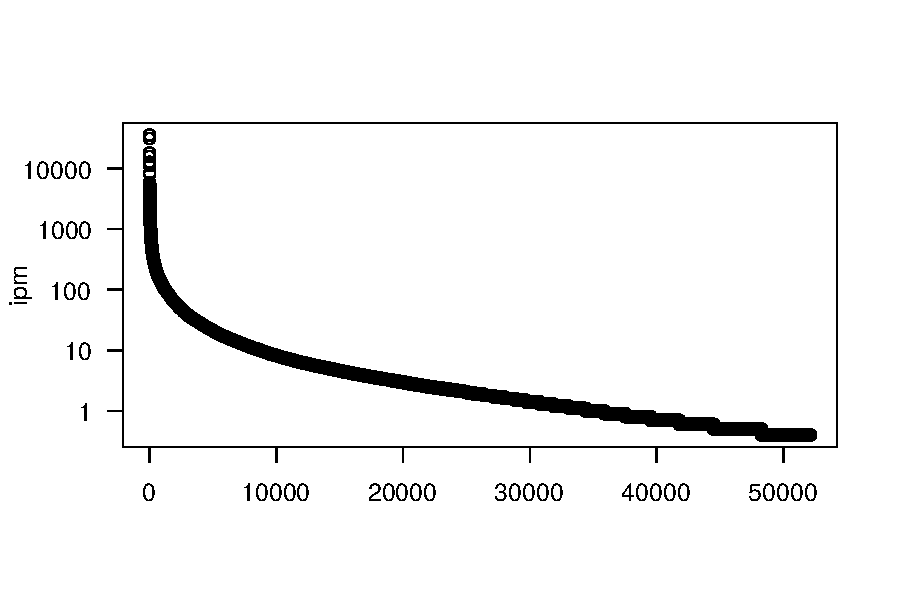
\includegraphics[width=0.49\linewidth]{016-base-scaterplot-log.pdf}~
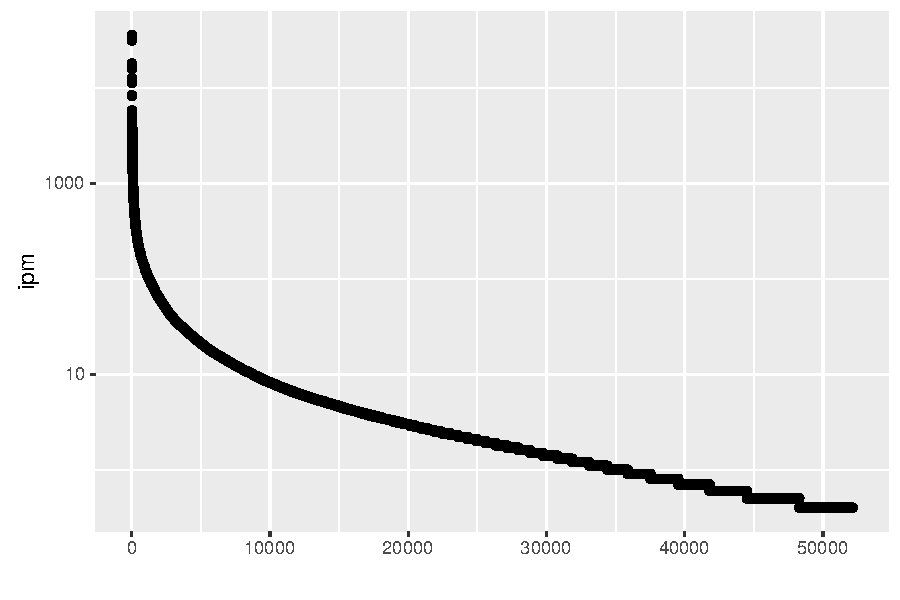
\includegraphics[width=0.49\linewidth]{016-ggplot-scaterplot-log.pdf}
\codel{
\# base R\\
plot(1:52138, freq\$Freq.ipm.,\\
\ \ \ xlab = NA, ylab = "ipm"{},\\
\ \ \ \alert{las = 1, \hfill \# поворот значений на оси y\\
\ \ \ log = "y"})\bigskip\\
\# dplyr, ggplot2\\
freq \%>\% \\
\ \ \ ggplot(aes(1:52138, Freq.ipm.))+\\
\ \ \ geom\_point()+\\
\ \ \ xlab("{}")+\\
\ \ \ ylab("ipm")+\\
\ \ \ \alert{scale\_y\_log10()} 
}
\end{frame}
\subsection{колич+катег}
\section{1 переменная}
\subsection{количественная}
\subsection{категориальная}
\section{3 переменные}
\subsection{колич+колич+колич}

\section{фасетизация}
\section{}
\begin{frame}
{\huge Спасибо что долистали!\bigskip\\
\normalsize Пишите письма\\
agricolamz@gmail.com
\vspace{-130pt}}
\end{frame}
\end{document}